\documentclass{beamer}

\usepackage{graphicx}
\usepackage{listings}
\usepackage{textpos}

\begin{document}

\beamertemplatenavigationsymbolsempty

\title{Digital Signal Processors}
\subtitle{Uses, Performance, Comparison to Traditional MCUs and FPGAs}
\author{Dinker Ambe\\
    John Collins\\
Alec Ten Harmsel}
\date{}

\addtobeamertemplate{frametitle}{}{%
    \begin{textblock*}{70mm}(.96\textwidth,-0.75cm)
        
\includegraphics[clip=true,width=0.20\textwidth]{m.png}
    \end{textblock*}
}

\frame{\titlepage}

\begin{frame}{Why Use a DSP?}
    \begin{itemize}
        \item Need to be able to watch 1080p video at 30Hz
            \begin{itemize}
                \item De-muxing video from cable/antenna
                \item Transform to video out to TV
                \item Ridiculously parallel problem
                \item Repetive math
                \item Real-time; around 3.33ms per frame
            \end{itemize}
        \item Much more power efficient than an MPU or CPU
            \begin{itemize}
                \item Many DSP chips can execute an FFT loop in 1 clock cycle
                \item The same FFT loop implementation on an MPU takes 29
                    instructions
                \item A modern DSP chip can transcode video at the same speed
                    as a high-range computer for a fraction of the price and
                    power
            \end{itemize}
        \item Much more flexible than an FPGA
            \begin{itemize}
                \item DSP chips are similar to an FPGA ``with batteries
                    included''
                \item Standard ISA, special memory architecture, etc.
            \end{itemize}
    \end{itemize}
\end{frame}

\begin{frame}{Uses}
    \begin{itemize}
        \item Real-time data transformation
            \begin{itemize}
                \item Cable box
                \item Audio receiver
                \item Automotive sensing
                \item Network switching
            \end{itemize}
        \item High throughput, low power data transformation
            \begin{itemize}
                \item Audio/video transcoding
                \item Cryptocurrency mining
            \end{itemize}
        \item Not for running a "modern" operating system % No virtual memory
        \item Not for generic workloads % Can't take advantage of hardware
    \end{itemize}
\end{frame}

\begin{frame}{History}
    \begin{itemize}
        \item Need for a solution that can execute complex math required for
            DSP
        \item Originally, DSP applications implemented using bit-slice
            processors
        \item First DSP created by TI in 1978, used in Speak \& Spell
            children's toy
        \item Second generation ~(80s) processors become standalone devices
        \item Third generation ~(90s) procesors allow hardware acceleration for
            complex math
        \item Fourth generation (current), higher clock speeds, smaller
            packaging, reduced price
    \end{itemize}
\end{frame}

\begin{frame}{Typical DSP Hardware}
    \begin{itemize}
        \item Parallel multipliers
        \item Parallel ALUs
        \item Parallel DMA memory controller
        \item Shifter
        \item Dedicated FFT hardware
        \item Example: Analog Devices' Blackfin Architecture
            \begin{itemize}
                \item 2x 16-bit MACs
                \item 2x 40-bit ALUs
                \item 4x 8-bit ALUs
                \item 1x 40-bit Shifter
            \end{itemize}
        \item Example: Texas Instruments' TMS320C55x Architecture
            \begin{itemize}
                \item 2x 16-bit MACs
                \item 1x 40-bit ALU
                \item 1x 16-bit ALU
            \end{itemize}
    \end{itemize}
\end{frame}

\begin{frame}{DSP Hardware Benefits}
    \begin{itemize}
        \item Real-time and low-latency
            \begin{itemize}
                \item Most DSP algorithms must be performed on a lot of incoming data
                \item Must be calculated repeatedly
                \item Used when there is a constrained time limit for calculations
                    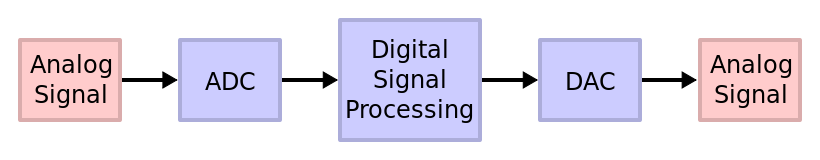
\includegraphics[width=0.6\textwidth]{block_diagram.png}
            \end{itemize}
        \item Can perform add, sub, mult, and div quickly and in parallel
        \item Parallel load, store
        \item Wide range of power and performance (Texas Instruments)
            \begin{itemize}
                \item Ultra-low power 16-bit with FFT acceleration (300 MHz)
                \item Power Optimized 32-bit fixed/float DSP (1+ GHz)
                \item High performance multicore 32-bit accellerated DSP (16 GHz)
            \end{itemize}
    \end{itemize}
\end{frame}

\begin{frame}{ISA}
    \begin{itemize}
        \item Mostly math instructions
        \item Special instructions
            \begin{itemize}
                \item MAC (Multiply accumulate)
                \item FIR (FIR filter)
                \item Square Distance
            \end{itemize}
        \item Typically can have two (or more) opcodes in an instruction for
            math instructions
        \item Few features: small interrupt table, no MMU, etc.
    \end{itemize}
    % Blackfins only have 7 or 9 configurable interrupts
    % MPUs are common, but no MMU for virtual memory
    % Typically have kernel and user mode
    % Parallel MAC, parallel math and store, etc.
\end{frame}

% Plots only show fixed point, 16-bit MAC units. This is a litte biased, since
% everything high-performance from TI is floating point.
\begin{frame}{Performance vs. Price}
    \begin{center}
        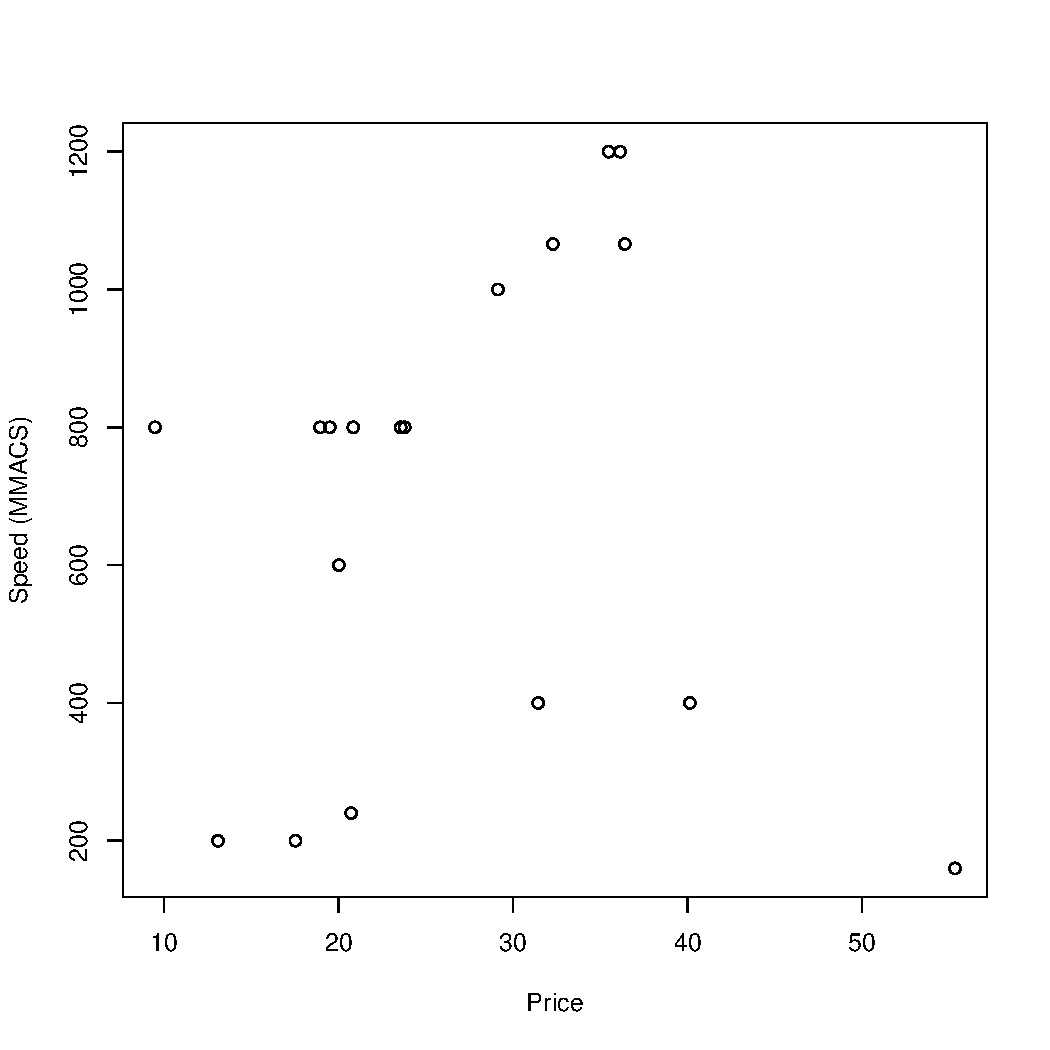
\includegraphics[width=0.8\textwidth]{price_perf.pdf}
    \end{center}
    % TI outlier is due to non-pipelined arch
    % Discuss pipelining and amortized single-cycle MACs
\end{frame}

\begin{frame}{Performance vs. Power}
    \begin{center}
        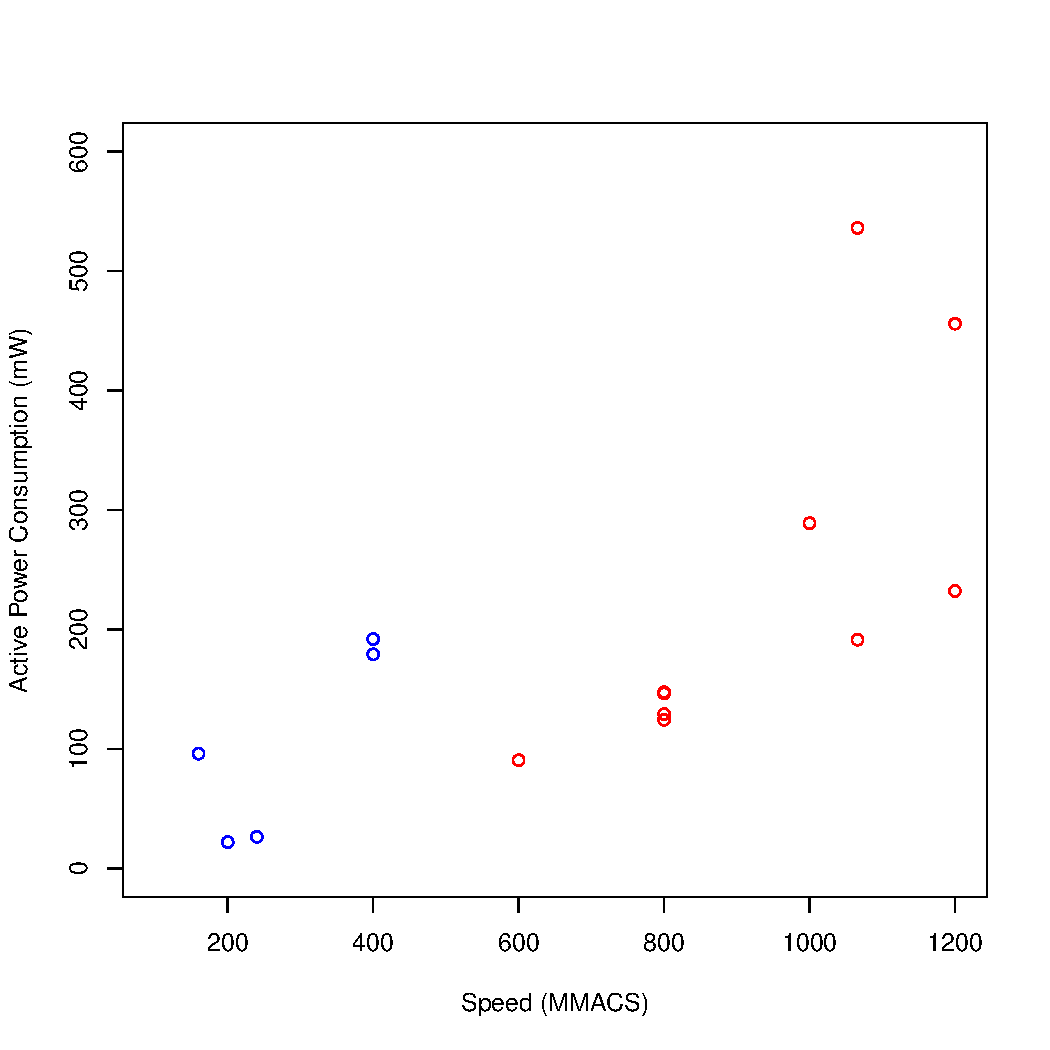
\includegraphics[width=0.8\textwidth]{power_perf.pdf}
    \end{center}
\end{frame}

\begin{frame}{How To Program a DSP}
    \begin{itemize}
        \item Architecture Description
            \begin{itemize}
                \item All available memory
                \item Memory mapped to external peripherals
            \end{itemize}
        \item Source Code Generation
            \begin{itemize}
                \item Slow but easy: High level languages such as C
                \item Fast but difficult: processor's native assembly
                \item Compromise: High level for generic functions, assembly for DSP computations
            \end{itemize}
    \end{itemize}
\end{frame}

\begin{frame}{FIR Filter in C}
    \begin{center}
        {\tiny
            \lstinputlisting{fir_example.c}
        }
    \end{center}
\end{frame}

\begin{frame}{FIR Filter in Assembly}
    \begin{center}
        {\tiny
            \lstinputlisting[firstline=52]{fir_example.s}
        }
    \end{center}
    % This is only the FIR part of the assembly. No interrupt setup or other
    % setup is shown.
\end{frame}

\begin{frame}{FIR in Assembly in a C program}
    \begin{center}
        {\tiny
            \lstinputlisting[firstline=36]{fir_asc_example.c}
        }
    \end{center}
\end{frame}

\end{document}
